\documentclass[10pt,letterpaper]{article}
\usepackage[square,comma,numbers]{natbib}
\usepackage{multibib}
\usepackage{xstring}
\usepackage{graphicx}
\usepackage{amsmath}

\usepackage{etoolbox}
\BeforeBeginEnvironment{thebibliography}{%
  \let\origsection\section% save the original definition of \section
  \let\section\subsection%  make \section behave like \subsection
}
\AfterEndEnvironment{thebibliography}{%
  \let\section\origsection% restore the original definition of \section
}


%\usepackage{hyperref}
%\usepackage[hidelinks]{hyperref}
\usepackage{color,hyperref}
\definecolor{darkblue}{rgb}{0.0,0.0,0.5}
\definecolor{myblue}{rgb}{0.0,0.0,1.0}
\definecolor{pink}{rgb}{1.0,0.1,0.8}
\hypersetup{colorlinks,breaklinks,linkcolor=blue,
  urlcolor=darkblue,anchorcolor=darkblue,citecolor=myblue}
\usepackage{enumitem}
\setlist[description]{
%   leftmargin=\parindent,
  leftmargin=0cm,
%   labelindent=0.3cm,
  labelindent=0cm,
  itemsep=1pt,
  %parsep=0pt,
  topsep=0pt,
}

\newcites{conf}{Conference Proceedings}

% \usepackage[colorlinks=false]{hyperref}  
\usepackage{geometry}
%\hypersetup{colorlinks=true}
%\usepackage[none]{hyphenat}

% Set your name here
\def\name{\textsc{Wen Xu}}

% The following metadata will show up in the PDF properties
\hypersetup{
  colorlinks = true,
  % urlcolor = black,
  pdfauthor = {\name},
  pdfkeywords = { Wen Xu, CV},
  pdftitle = {\name: Curriculum Vitae},
  pdfsubject = {Curriculum Vitae},
  pdfpagemode = UseNone
}

\geometry{
  body={6.5in, 9.0in},
  left=1.0in,
  top=1.0in
}

% highlight myname in bibliography
\def\FormatName#1{%
  \def\myname{Wen Xu}%
  \edef\name{#1}%
  \ifx\name\myname
    \underline{#1}%
  \else
    #1%
  \fi
}

% insert newline between bib items
\def\FormatRET{%
  \\%
}

% bold paper titles in bibliography
\def\FormatTitle#1{%
  \textbf{#1}%
}

% highlight awards.
\def\FormatNote#1{%
  #1%
}

% Customize page headers
% \pagestyle{myheadings}
% \markright{\name}
\thispagestyle{empty}

% Custom section fonts
\usepackage{sectsty}
% \sectionfont{\rmfamily\mdseries\Large}
% \subsectionfont{\rmfamily\mdseries\itshape\large}

% \sectionfont{\rmfamily\mdseries\Large\textbf}
% \subsectionfont{\rmfamily\mdseries\large\textbf}

% Other possible font commands include:
% \ttfamily for teletype,
% \sffamily for sans serif,
% \bfseries for bold,
% \scshape for small caps,
% \normalsize, \large, \Large, \LARGE sizes.

% Don't indent paragraphs.
\setlength\parindent{0em}

% Make lists without bullets and compact spacing
\renewenvironment{itemize}{
  \begin{list}{}{
    \setlength{\leftmargin}{3.5em}
    \setlength{\itemsep}{0.25em}
    \setlength{\parskip}{0pt}
    \setlength{\parsep}{0.25em}
  }
}{
  \end{list}
}

% bib heading: References -> Publication
\renewcommand{\refname}{Publication}

% customize the \section command
\usepackage{titlesec} 
\titleformat{\section}{\Large\scshape\raggedright}{}{0em}{}[\titlerule] % Text formatting of sections
% \titlespacing{\section}{0pt}{3pt}{3pt} % Spacing around sections


\begin{document}

% Place name at left
{\Huge \name}

% Alternatively, print name centered and bold:
%\centerline{\huge \bf \name}

\vspace{0.15in}

\begin{minipage}[t]{0.45\textwidth}
  Postdoctoral Fellow\\
  School of Computer Science\\
  Georgia Institute of Technology\\
  756 West Peachtree Street NW\\
  Atlanta, GA 30332-4016
\end{minipage}
\begin{minipage}[t]{0.45\textwidth}
  Email: \texttt{wen.xu@gatech.edu} \\
  Web: \url{https://gts3.org/~wen} \\
\end{minipage}

% \begin{minipage}[b]{0.35\textwidth}
  Postdoctoral Fellow\\
  School of Computer Science\\
  Georgia Institute of Technology\\
  Room 3138, 266 Ferst Dr NW\\
  Atlanta, GA 30332-0765
\end{minipage}
\begin{minipage}[b]{0.42\textwidth}
  Phone: (678) 469-6810\\
  Email: \texttt{sangho@gatech.edu} \\
  Web: \url{https://cc.gatech.edu/~slee3036}
\end{minipage}
\begin{minipage}[b]{0.18\textwidth}
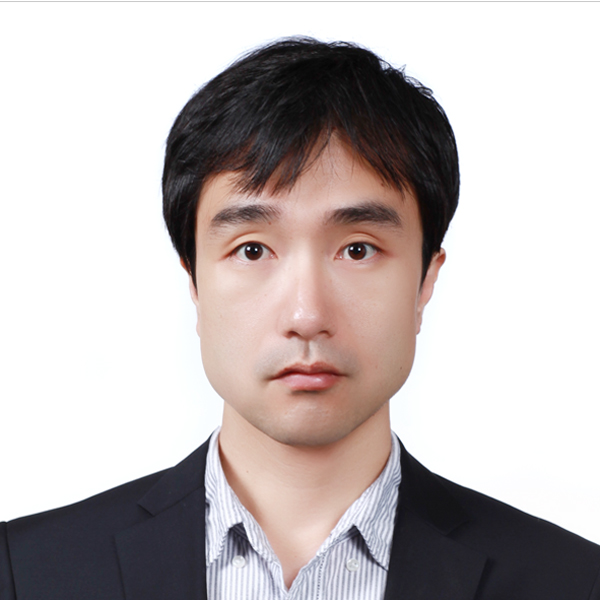
\includegraphics[width=\textwidth]{sangho.jpg}
\end{minipage}


\section*{Employment}

\begin{description}
\item {\bf Georgia Institute of Technology}, Atlanta, GA
\dotfill August 2016--Present
  \begin{itemize}
  \item Research Assistant
  \item Advisor: Dr. Taesoo Kim
  \end{itemize}

 \item {\bf Microsoft}, Redmond, WA \dotfill May 2019--July 2019
  \begin{itemize}
  \item Security Researcher
  \item Offensive Security Research (OSR) Team, Platform Security
  \end{itemize}
 
\item {\bf Microsoft Research}, Redmond, WA \dotfill May 2017--August 2017
  \begin{itemize}
  \item Research Intern
  \item Advisor: Marcus Peinado
  \end{itemize}

\item {\bf Singapore Management University}, Singapore \dotfill August 2015--February 2016
  \begin{itemize}
  \item Research Assistant
  \item Advisor: Dr. Xuhua Ding
  \end{itemize}

\item {\bf Tencent KeenLab (previously Keen Team)}, Shanghai, China \dotfill July 2014--June 2016
	\begin{itemize}
	\item Security Research Intern
	\end{itemize}
\end{description}

\section*{Education}

\begin{description}
\item {\bf Georgia Institute of Technology}, Atlanta, GA \dotfill August 2016--July 2021
  \begin{itemize}
  \item Ph.D. in Computer Science
  \item Advisor: Dr. Taesoo Kim
  \end{itemize}
  
\item {\bf Shanghai Jiao Tong University}, Shanghai, China \dotfill September 2012--June 2016
  \begin{itemize}
  \item B.S.E. in Computer Science
  \item ACM Honored Class
  \end{itemize}

\end{description}

\section*{Research Interests}
\begin{description}
\item Fuzzing, Systems Security
\end{description}


\section*{Publications} 

%%%%%%%%%%%%%%%%%%%%%%%%%%%%%%%%%%%%%%%
% Conference
\setlength{\bibsep}{5pt}
% \bibliographystyleconf{mybibstyle}
\bibliographystyleconf{plainyr}

\nociteconf{ding:snap, xu:freedom, park:die, ding:desensitization, kim:hydra, park:libmpk, xu:janus, xu:osfuzz, zhao:imee, kim:cabfuzz, xu:collide, xu:woot, xu:root, xu:sheriff}

\bibliographyconf{wen}

\section*{Presentations}
\begin{description}

    \item \textbf{An Advanced and Extensive Fuzzing Framework for File System Testing}
        \begin{itemize}
            \item Google, Sunnyvale, CA \dotfill July 2019
        \end{itemize}

    \item \textbf{Fuzzing File Systems via Two-Dimensional Input Space Exploration}
        \begin{itemize}
            \item KAIST, South Korea \dotfill April 2019
        \end{itemize}

	\item \textbf{Comprehensive Browser Fuzzing: From DOM to JS}
      \begin{itemize}
          \item w/ Soyeon Park, ZeroCon 2019, South Korea \dotfill April 2019
      \end{itemize}

	\item \textbf{The Road of Growth of 0ops Team}
      \begin{itemize}
          \item Shanghai, China \dotfill April 2016
      \end{itemize}

	\item \textbf{From Collision To Exploitation: Unleashing Use-After-Free Vulnerabilities in Linux Kernel}
		\begin{itemize}
			\item Nanyang Technological University, Singapore \dotfill November 2015
		\end{itemize}

  \item \textbf{Root Hundreds of Thousands of Android Devices with One Generic Exploit}
    \begin{itemize}
      \item HITB GSEC, Singapore \dotfill October 2015
    \end{itemize}

\end{description}

\section*{Honors and Awards}
\begin{description}
\item Postdoctoral research fellowship by
  National Research Foundation of Korea (\$35,000 award), 2017

\item Runner-up prize by
  Evaluation of ITRC Support Program (\$1,000 award), 2013

\end{description}

\section*{Teaching Experience}
\begin{description}

\item Teaching Assistant, Information Security Lab (Georgia Tech), 2016

\end{description}

\section*{Reported Vulnerabilities}
\begin{description}
\item {\emph{Linux Kernel}}
    \item $\bullet$ \textbf{ext4}: CVE-2018-10883, CVE-2018-10882, CVE-2018-10881, CVE-2018-10880, CVE-2018-10879, CVE-2018-10878, CVE-2018-10877, CVE-2018-10876, CVE-2018-10840, CVE-2018-1095, CVE-2018-1094, CVE-2018-1093, CVE-2018-1092
    \item $\bullet$ \textbf{Btrfs}: CVE-2018-14613, CVE-2018-14612, CVE-2018-14611, CVE-2018-14610, CVE-2018-14609
    \item $\bullet$ \textbf{XFS}: CVE-2018-13095, CVE-2018-13094, CVE-2018-13093, CVE-2018-10323, CVE-2018-10322
    \item $\bullet$ \textbf{F2FS}: CVE-2018-14616, CVE-2018-14615, CVE-2018-14614, CVE-2018-13100, CVE-2018-13099, CVE-2018-13098, CVE-2018-13097, CVE-2018-13096
	\item $\bullet$ \textbf{HFS+}: CVE-2018-14617
	\item $\bullet$ \textbf{Network}: CVE-2015-3636 (w/ Shi Wu)

\item {\emph{Apple}}
\item $\bullet$ \textbf{Safari (WebKit)}: CVE-2019-6212,
CVE-2019-8562 (w/ Hanqing Zhao), CVE-2019-8596, CVE-2019-8609,
CVE-2019-8619 (w/ Hanqing Zhao), CVE-2019-8628 (w /Hanqing
Zhao), CVE-2019-8673 (w/ Soyeon Park), CVE-2019-8676 (w/ Soyeon
Park), CVE-2019-8720

\item {\emph{Google}}
\item $\bullet$ \textbf{Chrome}: CVE-2016-1646 (\$7.5K),CVE-2019-5806 (\$3K), CVE-2019-5817 (\$1K), Issue 943424 (beta/\$3K), Issue 943538 (beta/\$3K), CVE-2019-13730 (\$5K, w/ Soyeon Park), CVE-2019-13764 (w/ Soyeon Park)
    \item $\bullet$ \textbf{Android}: CVE-2015-6612 (w/ Qidan He)

\item {\emph{Microsoft}}
	\item $\bullet$ \textbf{Script engine (ChakraCore)}: CVE-2016-0193 (w/ Zhen Feng), CVE-2019-0609 (w/ Soyeon Park), CVE-2019-1023 (w/ Soyeon Park)

\item {\emph{Qualcomm}}
	\item $\bullet$ \textbf{Camera drivers}: CVE-2014-9410, CVE-2014-4324, CVE-2014-4321 (w/ Sen Nie, Shi Wu and Liang Chen)
\end{description}


% \section*{Open Source Contribution}

\begin{description}

\item
\textbf{T-SGX}. Protecting SGX enclaves from controlled-channel attacks~\citeconf{lee:tsgx}. Co-lead author.
\vspace{-0.12cm}
\begin{itemize}
\item \url{https://github.com/sslab-gatech/t-sgx}
\end{itemize}  

\item
\textbf{DrK}. PoC of TSX-based Kernel ASLR de-randomization attack~\citeconf{jang:drk}. Contributor.
\vspace{-0.12cm}
\begin{itemize}
\item \url{https://github.com/sslab-gatech/DrK}
\end{itemize}  

\end{description}

\section*{Public and Community Service}
\begin{description}
\item Organizer of 0CTF Hacking Competition (DEFCON CTF pre-qualifier since 2016) \dotfill 2014-2018
\item Co-founder of 0ops CTF Team \dotfill 2013
\end{description}


% \section*{List of References}

\begin{description}
    \item \textbf{Taesoo Kim} (Postdoc advisor)
      \begin{itemize}
        \setlength\itemsep{0.1pt}
        \item Assistant Professor of Computer Science
        \item Georgia Institute of Technology, Atlanta, GA
        \item Homepage: \url{http://taesoo.gtisc.gatech.edu}
        \item Email: taesoo@gatech.edu
      \end{itemize}
    \item \textbf{Wenke Lee} (Postdoc co-advisor)
      \begin{itemize}
        \setlength\itemsep{0.1pt}
        \item Professor of Computer Science
        \item Georgia Institute of Technology, Atlanta, GA
        \item Homepage: \url{http://wenke.gtisc.gatech.edu}
        \item Email: wenke@cc.gatech.edu
      \end{itemize}
    \item \textbf{Jong Kim} (Ph.D. advisor)
      \begin{itemize}
        \setlength\itemsep{0.1pt}
        \item Professor of Computer Science and Engineering
        \item POSTECH, Pohang, South Korea
        \item Homepage: \url{https://hpc.postech.ac.kr/~jkim}
        \item Email: jkim@postech.edu
      \end{itemize}
    \item \textbf{Marcus Peinado}
      \begin{itemize}
        \setlength\itemsep{0.1pt}
        \item Architect
        \item Microsoft Research. Redmond, WA 
        \item Homepage: \url{http://research.microsoft.com/en-us/people/marcuspe} 
        \item Email: marcuspe@microsoft.com
      \end{itemize}
    \item \textbf{Jangwoo Kim}
      \begin{itemize}
        \setlength\itemsep{0.1pt}
        \item Associate Professor of Electrical and Computer Engineering
        \item Seoul National University, Seoul, South Korea
        \item Homepage: \url{https://hpcs.snu.ac.kr/~jangwoo}
        \item Email: jangwoo@snu.ac.kr
      \end{itemize}

\end{description}

% \input{other}

% Footer

\begin{center}
  \begin{small}
    Last updated: \today
  \end{small}
\end{center}

\end{document}



